\section{Methodology}
\label{sec:methodology}

As already alluded to in \autoref{sec:introduction} the goal of the project is to
analyse commit messages. To achieve this repositories of the top 10 most
wanted languages were used. This list was used as a reference, since it
has a great assortment of languages that are in high demand and also relevant
in today's development climate. The languages in question are:

\begin{figure}[H]
  \centering
  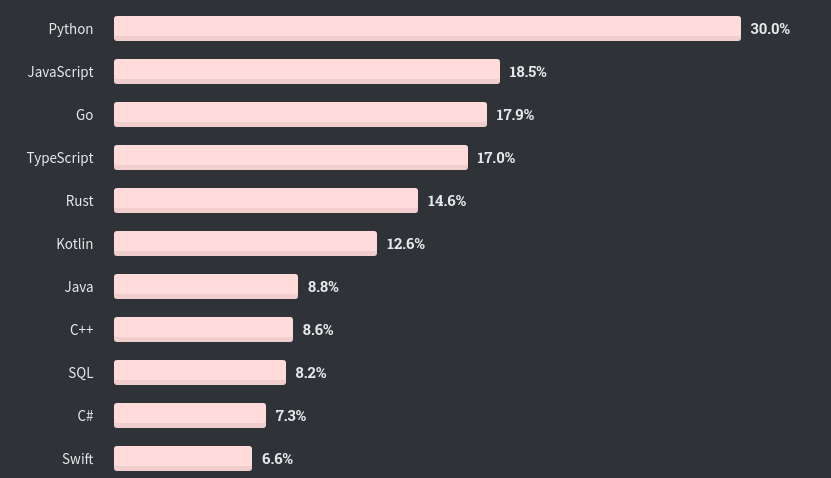
\includegraphics[width=\textwidth]{wanted_languages.png}
  \caption{top 10 most wanted languages \cite{so-survey}}
  \label{fig:wanted_languages}
\end{figure}

It has to be noted that not all languages depicted in
\autoref{fig:wanted_languages} have been chosen since SQL is a query language
and not considered a general programming language. As SQL it is not
suited to be used as a main repository language, Swift has been chosen instead.
Regardless of the percentages seen in \autoref{fig:wanted_languages}, 100000 commits of each
language have been considered for the final set, where 10000 is the maximum per
repository. To further diversify the results a limit has been imposed regarding
the amount of commits per author. This limit has been set to 100, since commit
messages by the same author are very likely to use a similar order of words,
even across different repositories. The authors are distinguished between their
e-mail addresses.

The language of choice for the programming part of the data set retrieval
is Python. Python is well suited for this project as it has rich support for
natural language processing related tasks. Additionally the language is great
for quick prototyping of ideas and with the help of tools like Jupyter
Notebook, documents with graphs and text can be created in no time. Especially
during the scraping process the library PyGithub was put to good use. PyGithub
is a Python library that offers typed interactions with the GitHub API v3
\cite{pygithub}. The results of the fetching process are furthermore cached in
one CSV file per language. As those files used the same format and headers, they
can easily be combined into one large file for convenience. However, one might
add the language as an additional column to not lose this information.

The data set was analysed using the NLKT library \cite{nltk} and Python.
The library was used to generate different word distributions and process
the messages themselves.

Since some repositories contain commits that are already tagged with some label,
regular expressions were used to filter a subset of those commits.
This subset was used to test a basic classification approach. The idea is to
determine how good a simple approach, only based on text analysis, actually is.

For the classification approach, the logistic regression implementation from
the Python module sklearn \cite{sklearn} was used. All previously filtered
labels were used to generate a common set of labels to be encoded for the
generation of feature vectors. The validation of the classifier was done using
10-Fold cross-validation.
